\let\negmedspace\undefined
\let\negthickspace\undefined
\documentclass[journal]{IEEEtran}
\usepackage[a5paper, margin=10mm, onecolumn]{geometry}
%\usepackage{lmodern} % Ensure lmodern is loaded for pdflatex
\usepackage{tfrupee} % Include tfrupee package

\setlength{\headheight}{1cm} % Set the height of the header box
\setlength{\headsep}{0mm}     % Set the distance between the header box and the top of the text

\usepackage{gvv-book}
\usepackage{gvv}
\usepackage{cite}
\usepackage{amsmath,amssymb,amsfonts,amsthm,mathtools}
\usepackage{algorithmic}
\usepackage{graphicx}
\usepackage{textcomp}
\usepackage{xcolor}
\usepackage{txfonts}
\usepackage{listings}
\usepackage{enumitem}
\usepackage{mathtools}
\usepackage{gensymb}
\usepackage{comment}
\usepackage[breaklinks=true]{hyperref}
\usepackage{tkz-euclide} 
\usepackage{listings}
\def\inputGnumericTable{}                                 
\usepackage[latin1]{inputenc}                                
\usepackage{color}                                            
\usepackage{array}                                            
\usepackage{longtable}                                       
\usepackage{calc}                                             
\usepackage{multirow}                                         
\usepackage{hhline}                                           
\usepackage{ifthen}                                           
\usepackage{lscape}
\begin{document}

\bibliographystyle{IEEEtran}
\vspace{3cm}

\title{3.3.2.25}
\author{EE24BTECH11024 - G. Abhimanyu Koushik
}
% \maketitle
% \newpage
% \bigskip
{\let\newpage\relax\maketitle}

\renewcommand{\thefigure}{\theenumi}
\renewcommand{\thetable}{\theenumi}
\setlength{\intextsep}{10pt} % Space between text and floats

\textbf{Question:}\\
A Triangle $ABC$ can be constructed in which $\angle B=60\degree$, $\angle C=45\degree$ and $AB+BC+CA=12cm$
\textbf{Solution:}
\begin{table}[h!]    
  \centering
  \begin{tabular}[12pt]{ |c|c|c|}
    \hline
    \textbf{Symbol} & \textbf{Value} & \textbf{Description} \\
    \hline
    $\vec{A}$ & \myvec{6\\5} & First point\\
    \hline 
    $\vec{B}$ & \myvec{-4\\3} & Second point\\
    \hline
    $\vec{Y}$ & \myvec{0\\$y$} & Point on Y-Axis equidistant from A and B\\
    \hline
    \end{tabular}

  \caption{Variables Used}
  \label{tab10.5.3.9.1}
\end{table}\\
From properties of triangles we get the following equations
\begin{align}
a+b+c&=K\\
a&=b\cos(C)+c\cos(B)\\
\frac{b}{\sin(B)}&=\frac{c}{\sin(C)}
\end{align}
Rewriting the equations will give
\begin{align}
	a+b+c&=K\\
	b\cos(C)+c\cos(B)-a&=0\\
	b\sin(C)-c\sin(B)&=0\\
\end{align}
It results in the following matrix equation
\begin{align}
  \myvec{1 & 1 & 1\\-1 & \cos(C) & \cos(B)\\0 & \sin(C) & -\sin(B)}\times\myvec{a\\b\\c}&=K\myvec{1\\0\\0}
\end{align}
We can find all the side lengths by solving the above matrix equation.
\begin{align}
  \myvec{1 & 1 & 1\\-1 & \frac{1}{\sqrt{2}} & \frac{1}{2}\\0 & \frac{1}{\sqrt{2}} & -\frac{\sqrt{3}}{2}}\times\myvec{x\\y\\z}&=\myvec{1\\0\\0}\\
  \myvec{1 & 1 & 1 & 1\\-1 & \frac{1}{\sqrt{2}} & \frac{1}{2} & 0\\0 & \frac{1}{\sqrt{2}} & -\frac{\sqrt{3}}{2} & 0} \xleftrightarrow[]{R_2 \leftarrow {R_1+R_2}}\myvec{1 & 1 & 1 & 1\\0 & \frac{1}{\sqrt{2}}+1 & \frac{3}{2} & 1\\0 & \frac{1}{\sqrt{2}} & -\frac{\sqrt{3}}{2} & 0}\\
  \xleftrightarrow[]{R_3 \leftarrow {R_2-\brak{\sqrt{2}+1}R_3}}\myvec{1 & 1 & 1 & 1\\0 & \frac{1}{\sqrt{2}}+1 & \frac{3}{2} & 1\\0 & 0 & \brak{\sqrt{3}+\sqrt{2}+1}\frac{\sqrt{3}}{2} & 1}\\
  \xleftrightarrow[]{R_3 \leftarrow {\brak{\frac{2}{\sqrt{3}\brak{\sqrt{3}+\sqrt{2}+1}}}R_3}}\myvec{1 & 1 & 1 & 1\\0 & \frac{1}{\sqrt{2}}+1 & \frac{3}{2} & 1\\0 & 0 & 1 & \frac{2}{\sqrt{3}\brak{\sqrt{3}+\sqrt{2}+1}}}\\
  \xleftrightarrow[]{R_2 \leftarrow {R_2-\brak{\frac{3}{2}}R_3}}\myvec{1 & 1 & 1 & 1\\0 & \frac{1}{\sqrt{2}}+1 & 0 & \frac{\sqrt{2}+1}{\sqrt{3}+\sqrt{2}+1}\\0 & 0 & 1 & \frac{2}{\sqrt{3}\brak{\sqrt{3}+\sqrt{2}+1}}}\\
  \xleftrightarrow[]{R_2 \leftarrow \brak{\frac{\sqrt{2}}{\sqrt{2}+1}}R_2}\myvec{1 & 1 & 1 & 1\\0 & 1 & 0 & \frac{\sqrt{2}}{\sqrt{3}+\sqrt{2}+1}\\0 & 0 & 1 & \frac{2}{\sqrt{3}\brak{\sqrt{3}+\sqrt{2}+1}}}\\
  \xleftrightarrow[]{R_1 \leftarrow R_1-R_2}\myvec{1 & 0 & 1 & \frac{\sqrt{3}+1}{\sqrt{3}+\sqrt{2}+1}\\0 & 1 & 0 & \frac{\sqrt{2}}{\sqrt{3}+\sqrt{2}+1}\\0 & 0 & 1 & \frac{2}{\sqrt{3}\brak{\sqrt{3}+\sqrt{2}+1}}}\\
  \xleftrightarrow[]{R_1 \leftarrow R_1-R_3}\myvec{1 & 0 & 0 & \frac{1+\sqrt{3}}{\sqrt{3}\brak{\sqrt{3}+\sqrt{2}+1}}\\0 & 1 & 0 & \frac{\sqrt{2}}{\sqrt{3}+\sqrt{2}+1}\\0 & 0 & 1 & \frac{2}{\sqrt{3}\brak{\sqrt{3}+\sqrt{2}+1}}}\\
\end{align}
The values of $x$,$y$,$z$ are
\begin{align}
x&=\frac{1+\sqrt{3}}{\sqrt{3}\brak{\sqrt{3}+\sqrt{2}+1}}\\
y&=\frac{\sqrt{2}}{\sqrt{3}+\sqrt{2}+1}\\
z&=\frac{2}{\sqrt{3}\brak{\sqrt{3}+\sqrt{2}+1}}
\end{align}
The values of $\frac{a}{K}$,$\frac{b}{K}$ and $\frac{c}{K}$ are
\begin{align}
\frac{a}{K}&=\frac{1+\sqrt{3}}{\sqrt{3}\brak{\sqrt{3}+\sqrt{2}+1}}\\
\frac{b}{K}&=\frac{\sqrt{2}}{\brak{\sqrt{3}+\sqrt{2}+1}}\\
\frac{c}{K}&=\frac{2}{\sqrt{3}\brak{\sqrt{3}+\sqrt{2}+1}}
\end{align}
The length of sides of triangle are
\begin{align}
a&=\frac{12+12\sqrt{3}}{\sqrt{3}\brak{\sqrt{3}+\sqrt{2}+1}}\\
b&=\frac{12\sqrt{2}}{\brak{\sqrt{3}+\sqrt{2}+1}}\\
c&=\frac{24}{\sqrt{3}\brak{\sqrt{3}+\sqrt{2}+1}}
\end{align}
\begin{figure}[h!]
   \centering
   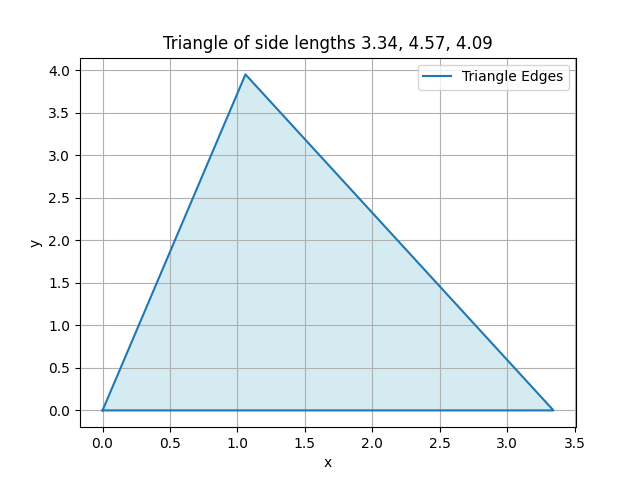
\includegraphics[width=0.7\linewidth]{figs/fig.png}
   \caption{Triangle with $\angle B=60\degree$, $\angle C=45\degree$ and Perimeter = $12cm$}
\end{figure}
\end{document}
